\documentclass{article}
\usepackage{pgfplots}
\usepackage{pifont}
\begin{document}

\begin{tikzpicture}
\begin{axis}
\addplot[color=red]{exp(x)};
\end{axis}
\end{tikzpicture}
%Here ends the furst plot
\hskip 5pt
%Here begins the 3d plot
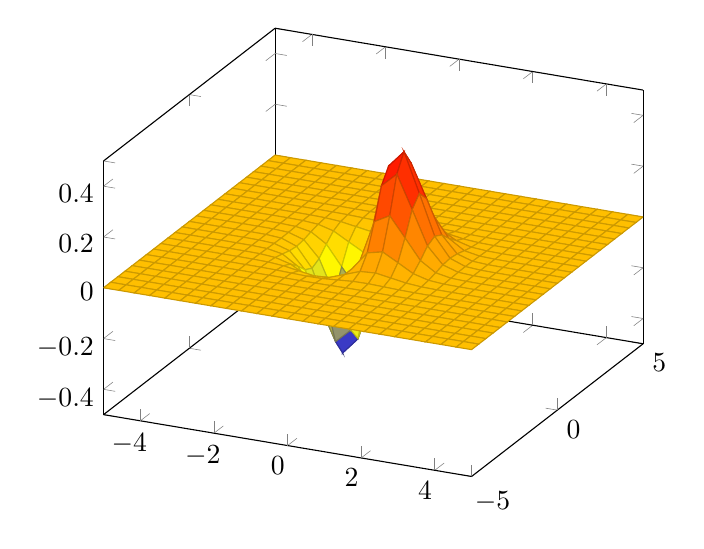
\begin{tikzpicture}
\begin{axis}
\addplot3[
    surf,
]
{exp(-x^2-y^2)*x};
\end{axis}
\end{tikzpicture}
\ding{172}
\end{document}
